% This file was created by tikzplotlib v0.8.5.
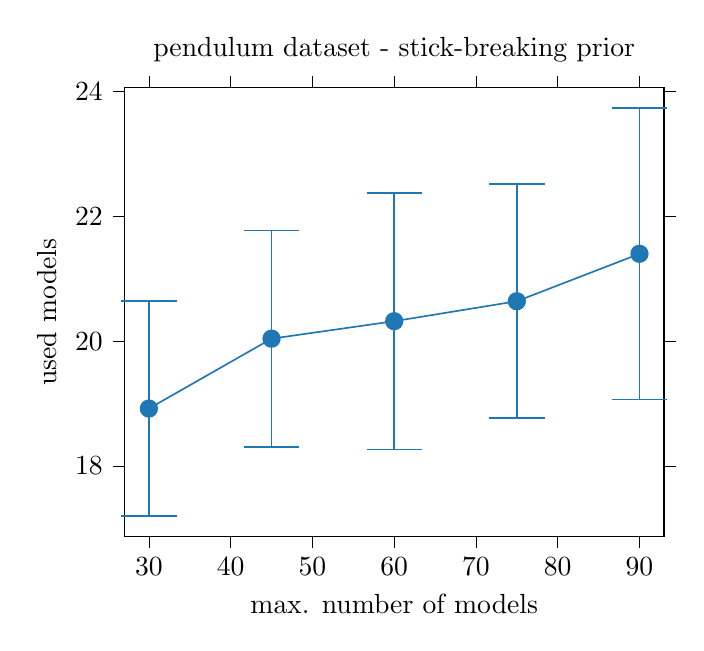
\begin{tikzpicture}

\definecolor{color0}{rgb}{0.12156862745098,0.466666666666667,0.705882352941177}

\begin{axis}[
tick align=outside,
tick pos=both,
title={pendulum dataset - stick-breaking prior },
x grid style={white!69.01960784313725!black},
xlabel={max. number of models},
xmin=27, xmax=93,
xtick style={color=black},
y grid style={white!69.01960784313725!black},
ylabel={used models},
ymin=16.8748466731521, ymax=24.0589300000708,
ytick style={color=black}
]
\path [draw=color0, semithick]
(axis cs:30,17.2013959152847)
--(axis cs:30,20.6386040847153);

\path [draw=color0, semithick]
(axis cs:45,18.3084111342469)
--(axis cs:45,21.7715888657531);

\path [draw=color0, semithick]
(axis cs:60,18.2663203755211)
--(axis cs:60,22.3736796244789);

\path [draw=color0, semithick]
(axis cs:75,18.7663938514191)
--(axis cs:75,22.5136061485809);

\path [draw=color0, semithick]
(axis cs:90,19.0676192420619)
--(axis cs:90,23.7323807579381);

\addplot [semithick, color0, mark=-, mark size=10, mark options={solid}, only marks]
table {%
30 17.2013959152847
45 18.3084111342469
60 18.2663203755211
75 18.7663938514191
90 19.0676192420619
};
\addplot [semithick, color0, mark=-, mark size=10, mark options={solid}, only marks]
table {%
30 20.6386040847153
45 21.7715888657531
60 22.3736796244789
75 22.5136061485809
90 23.7323807579381
};
\addplot [semithick, color0, mark=*, mark size=3, mark options={solid}]
table {%
30 18.92
45 20.04
60 20.32
75 20.64
90 21.4
};
\end{axis}

\end{tikzpicture}
